\documentclass[11pt,a4paper]{article}

\usepackage[english]{babel}
\usepackage{amsmath}
\usepackage{amssymb}
\usepackage{booktabs}
\usepackage[a4paper,margin=2.5cm]{geometry}
\usepackage{microtype}
\usepackage[htt]{hyphenat}
\usepackage{graphicx}
\usepackage{float}
\usepackage{listings}
\usepackage{xcolor}
\usepackage{caption}
\usepackage[hidelinks]{hyperref}

\graphicspath{{figs/}}
\captionsetup{font=small,labelfont=bf}

\definecolor{codeblue}{HTML}{1F4E79}
\definecolor{codegreen}{HTML}{2E7D32}
\definecolor{codegray}{HTML}{6E6E6E}
\definecolor{codebg}{HTML}{F7F7F7}

\lstset{
  language=Python,
  basicstyle=\ttfamily\footnotesize,
  keywordstyle=\color{codeblue}\bfseries,
  commentstyle=\color{codegreen}\itshape,
  stringstyle=\color{red!60!black},
  numberstyle=\tiny\color{codegray},
  numbers=left,
  numbersep=8pt,
  backgroundcolor=\color{codebg},
  frame=single,
  rulecolor=\color{codegray},
  breaklines=true,
  breakatwhitespace=false,
  columns=fullflexible,
  keepspaces=true,
  showstringspaces=false,
  tabsize=2,
  captionpos=b,
  upquote=true
}

\title{\bfseries Applied Reinforcement Learning (A2C) on Transportation Stocks}
\author{handed in by\\[0.3em]Christopher Voizard}
\date{\today}

\begin{document}

\maketitle
\thispagestyle{empty}

\newpage
\tableofcontents
\newpage

\section{Introduction and Companies Selected}

As the subject of this study, I chose three companies more or less related to the
transportation industry, which for various reasons have had difficulties in recent
years, especially environment-related, to publish good business figures. The two
aircraft manufacturers \textbf{Boeing} and \textbf{Airbus}, which share the market
completely between themselves, were particularly affected by the lockdown during the
last pandemic and the shutdown. However, vehicle manufacturers such as market leader
\textbf{Toyota} are also facing changing market demand. In view of these challenges, it
is interesting to conduct an analysis of future performance and to compare buy-and-hold
strategies to our trained agent.

The following descriptive statistics are used to evaluate the performance of the shares:
\begin{itemize}
  \item share price over the last 10 years,
  \item price-earnings ratio (P/E ratio),
  \item price-to-sales ratio (P/S ratio),
  \item log-returns.
\end{itemize}

\paragraph{Price-earnings ratio (P/E ratio).}
The price/earnings ratio is the number of years in which the company would have earned
its stock market value if profits had remained constant. In the calculation, the current
share or stock market price is divided by the company's earnings per share. The
company's earnings per share are calculated by dividing the company's earnings by the
total number of shares. The common and relevant sites give a guideline value between 12
and 15 for the interpretation of the P/E ratio. If the results are below this value, a
share tends to be considered cheap; if the results are above 15, the share may tend to be
considered more expensive. The formula is
\begin{equation}
  P/E = \frac{\text{share price}}{\text{earnings per share}}.
\end{equation}

\paragraph{Price-to-sales ratio (P/S ratio).}
The price-to-sales ratio (P/S ratio) is a share ratio that shows the market value of a
share in relation to its annual sales. The lower the P/S compared to the values of other
companies in the same industry, the more favorable the respective share is. The common
and relevant sites give a guideline value above 1 and below 1 for the interpretation of
the P/S ratio. If the results are below this value, a share tends to be considered cheap;
if the results are above 1, the share may tend to be considered more expensive. It can be
calculated as follows:
\begin{equation}
  P/S_{total} = \frac{\text{sales}}{\text{market capitalisation}}.
\end{equation}

\paragraph{Log-returns.}
The log return can be calculated by simply taking a natural logarithm of the current
price $(p_1)$ divided by the initial price $(p_0)$:
\begin{equation}
  r_1 = \ln\!\left(\frac{p_1}{p_0}\right).
\end{equation}

\subsection{Share price over the last 10 years}

\begin{figure}[H]
  \centering
  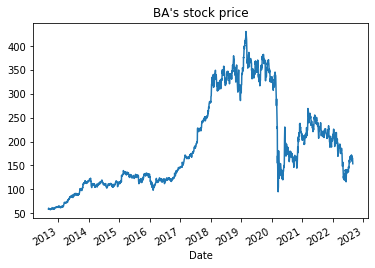
\includegraphics[width=0.62\textwidth]{z006_1.png}
  \caption{Boeing (BA) -- closing price over the last 10 years.}
\end{figure}

\begin{figure}[H]
  \centering
  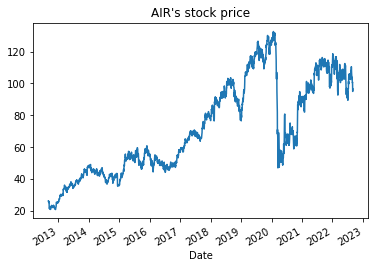
\includegraphics[width=0.62\textwidth]{z008_1.png}
  \caption{Airbus (AIR.PA) -- closing price over the last 10 years.}
\end{figure}

\begin{figure}[H]
  \centering
  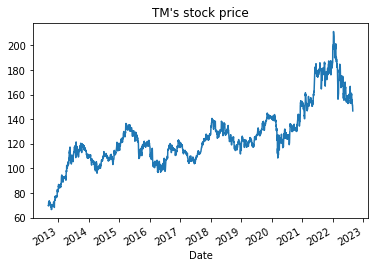
\includegraphics[width=0.62\textwidth]{z010_1.png}
  \caption{Toyota (TM) -- closing price over the last 10 years.}
\end{figure}

\paragraph{Comments.}
The price chart shows the time sequence on the abscissa and the price of the share on the
ordinate. Both Boeing and Airbus show a significant drop in price at the beginning of
2020, i.e.\ the first lockdown and the suspension of air traffic. While Airbus was almost
back to its previous high of 2020 at the beginning of 2022, Boeing shows a much more
negative trend. Toyota, on the other hand, reached its peak at the beginning of 2022, but
has also shown a negative trend since then.

\subsection{Price-earnings ratio (P/E ratio)}

The P/E values obtained for the three companies are summarised in Table~\ref{tab:pe}.

\begin{table}[H]
  \centering
  \caption{Price-earnings ratio (P/E).}
  \label{tab:pe}
  \begin{tabular}{lll}
    \toprule
    Company & P/E & Remark\\
    \midrule
    Boeing & -- & value not returned by the data source\\
    Airbus & 19.89 & \\
    Toyota & 10.37 & \\
    \bottomrule
  \end{tabular}
\end{table}

\paragraph{Comments.}
Given the P/E values for Airbus and Toyota of 19.9 and 10.4, respectively, it can be seen
that Airbus is above the guideline value of 15 and can thus be regarded as rather
expensive, while Toyota can be regarded as rather inexpensive by industry standards.

\subsection{Price-to-sales ratio (P/S ratio), last 12 months}

\begin{table}[H]
  \centering
  \caption{Price-to-sales ratio (P/S).}
  \label{tab:ps}
  \begin{tabular}{ll}
    \toprule
    Company & P/S\\
    \midrule
    Boeing & 1.502\\
    Airbus & 1.458\\
    Toyota & 0.006\\
    \bottomrule
  \end{tabular}
\end{table}

\paragraph{Comments.}
Similar to the P/S value above, it can be seen that both Boeing and Airbus are classified
as more or less expensive with values of 1.5 and 1.4 respectively, while Toyota could
even be classified as favorable with a value close to zero.

\subsection{Log-returns}

\begin{table}[H]
  \centering
  \caption{Cumulative log-returns over the observed period.}
  \label{tab:logret}
  \begin{tabular}{lrr}
    \toprule
    Company & Log-return & in \%\\
    \midrule
    Boeing & $-0.3025$ & $-30.2$\\
    Airbus & $-0.1451$ & $-14.5$\\
    Toyota & $-0.1486$ & $-14.9$\\
    \bottomrule
  \end{tabular}
\end{table}

\paragraph{Comments.}
The log return of the last year shows for all three stocks that a simple buy-and-hold
strategy would have led to more or less larger losses during this period. In the case of
Boeing with a loss of 30\%, in the case of Airbus with 14\% and for Toyota with a loss of
15\%.

\section{A2C Algorithm Applied and Analysis}

For each of the three shares, an Advantage Actor-Critic (A2C) agent was trained and
evaluated against a simple buy-and-hold strategy. Per share, five independently trained
agents were compared with the market. The tables below report the average returns of the
trained agents, the average returns of the market (buy and hold), and the average
percentage of cases in which the agent performed better than the market.

\subsection{Boeing}

\begin{table}[H]
  \centering
  \caption{Boeing -- average returns of agent vs.\ market.}
  \label{tab:boeing}
  \begin{tabular}{lrrrrr}
    \toprule
     & Agent 1 & Agent 2 & Agent 3 & Agent 4 & Agent 5\\
    \midrule
    Trained agent   & 1.151250 & 0.982355 & 1.268870 & 1.211902 & 1.220214\\
    Market (B\&H)   & 1.220214 & 1.194680 & 1.411054 & 1.325877 & 1.139906\\
    Agent better (\%) & 0.55 & 0.10 & 0.40 & 0.80 & 0.40\\
    \bottomrule
  \end{tabular}
\end{table}

\begin{figure}[H]
  \centering
  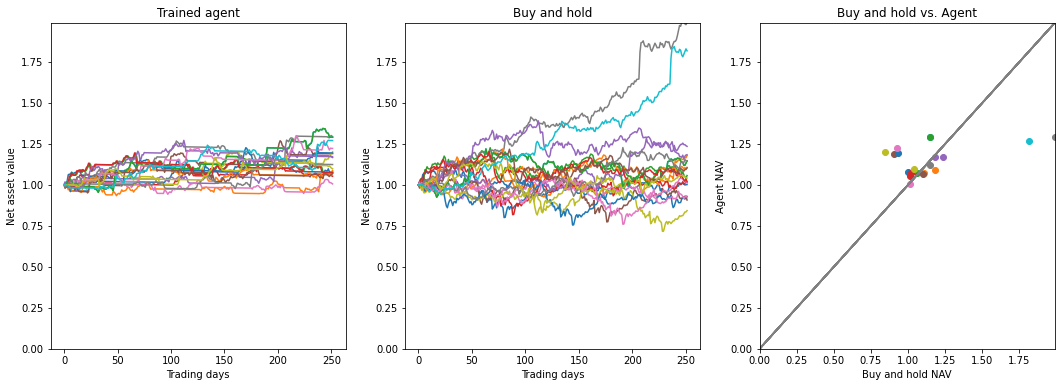
\includegraphics[width=0.78\textwidth]{z043_1.png}
  \caption{Boeing -- cumulative return ratio: buy and hold vs.\ trained agent.}
\end{figure}

\begin{figure}[H]
  \centering
  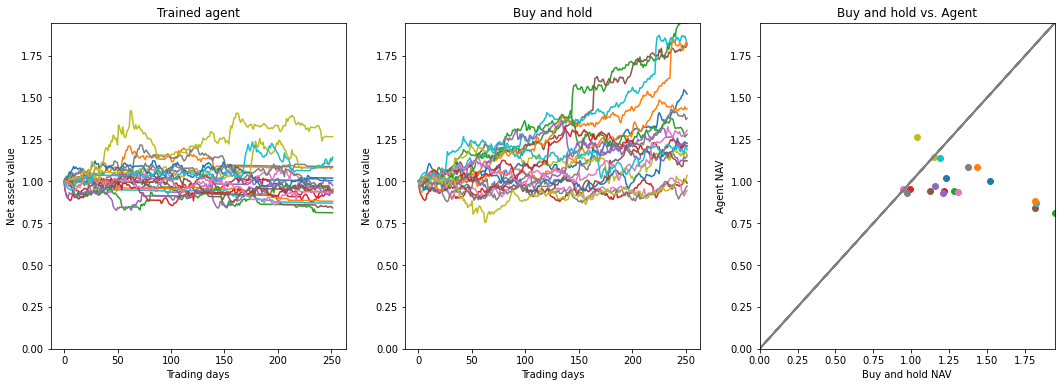
\includegraphics[width=0.78\textwidth]{z044_1.png}
  \caption{Boeing -- actions chosen by the trained agents over time.}
\end{figure}

\paragraph{Commentary on the result for Boeing.}
Given those numbers, it can be stated that the A2C algorithm applied to the Boeing share
would not result in an overall better performance than the simple buy-and-hold strategy.
Only in 45\% of the cases (on average) would the trained agent show a better performance.
This is mainly due to one entrained agent which leads to better results than the market in
only 10\% of the cases. The analysis of the performed actions shows significantly
different values, especially for the values for \emph{short} and \emph{cash}, distributed
among the trained agents. It can therefore be assumed that the trained agent applied to
this stock leads to inconsistent decisions and therefore to inconsistent and rather less
promising results.

\subsection{Airbus}

\begin{table}[H]
  \centering
  \caption{Airbus -- average returns of agent vs.\ market.}
  \label{tab:airbus}
  \begin{tabular}{lrrrrr}
    \toprule
     & Agent 1 & Agent 2 & Agent 3 & Agent 4 & Agent 5\\
    \midrule
    Trained agent   & 1.430267 & 1.570172 & 2.007212 & 1.276262 & 1.038152\\
    Market (B\&H)   & 1.217388 & 1.188968 & 1.168107 & 1.195885 & 1.237382\\
    Agent better (\%) & 0.75 & 0.60 & 0.80 & 0.60 & 0.20\\
    \bottomrule
  \end{tabular}
\end{table}

\begin{figure}[H]
  \centering
  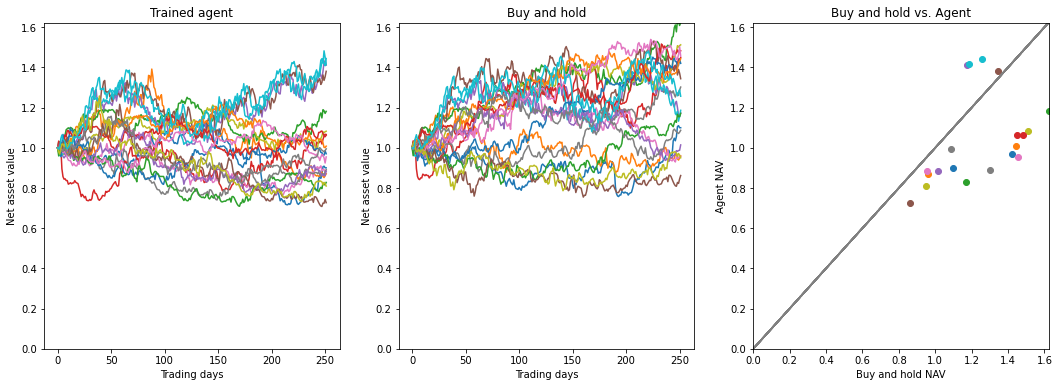
\includegraphics[width=0.78\textwidth]{z058_1.png}
  \caption{Airbus -- cumulative return ratio: buy and hold vs.\ trained agent.}
\end{figure}

\begin{figure}[H]
  \centering
  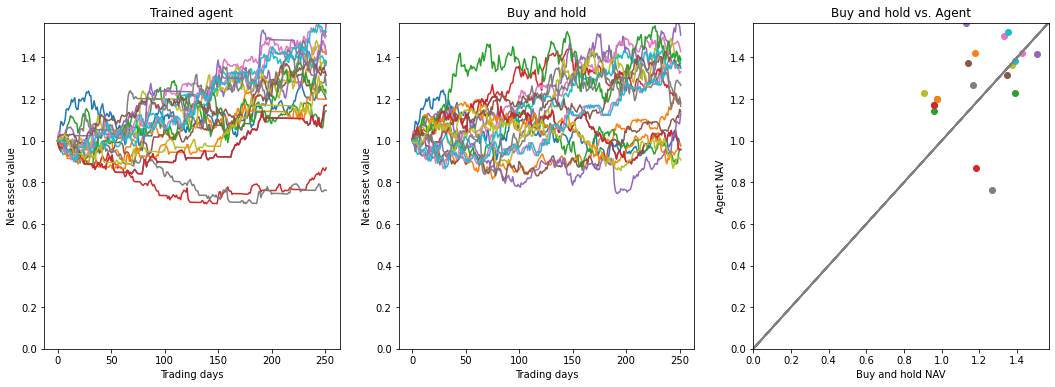
\includegraphics[width=0.78\textwidth]{z059_1.png}
  \caption{Airbus -- actions chosen by the trained agents over time.}
\end{figure}

\paragraph{Commentary on the result for Airbus.}
Given those numbers, it can be stated that the A2C algorithm applied to the Airbus share
would result in an overall better performance than the simple buy-and-hold strategy. In
60\% of the cases (on average) the trained agent would show a better performance. The
analysis of the performed actions shows similar values for four trained agents; only one
trained agent differs a lot in terms of \emph{cash}. It can therefore be assumed that the
trained agent applied to this share could lead to consistent and promising results.

\subsection{Toyota}

\begin{table}[H]
  \centering
  \caption{Toyota -- average returns of agent vs.\ market.}
  \label{tab:toyota}
  \begin{tabular}{lrrrrr}
    \toprule
     & Agent 1 & Agent 2 & Agent 3 & Agent 4 & Agent 5\\
    \midrule
    Trained agent   & 1.160707 & 1.442139 & 1.185587 & 1.263972 & 1.272148\\
    Market (B\&H)   & 0.994851 & 1.014057 & 1.044513 & 1.070050 & 1.003871\\
    Agent better (\%) & 0.80 & 0.70 & 0.80 & 0.85 & 0.75\\
    \bottomrule
  \end{tabular}
\end{table}

\begin{figure}[H]
  \centering
  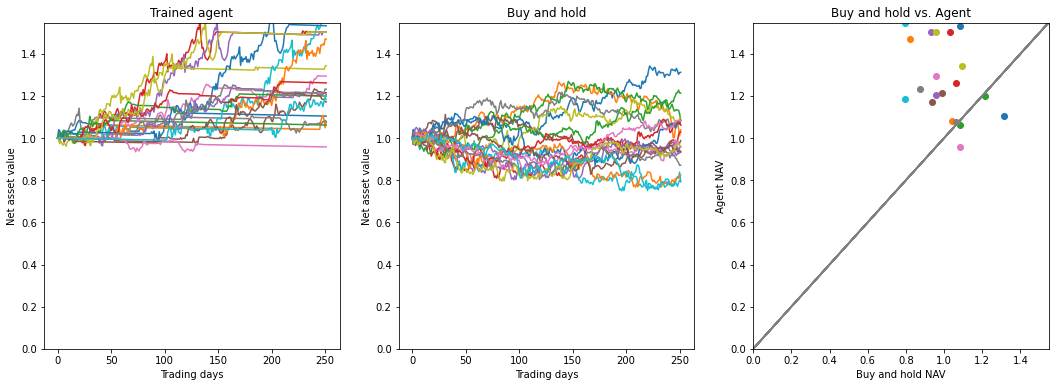
\includegraphics[width=0.78\textwidth]{z073_1.png}
  \caption{Toyota -- cumulative return ratio: buy and hold vs.\ trained agent.}
\end{figure}

\begin{figure}[H]
  \centering
  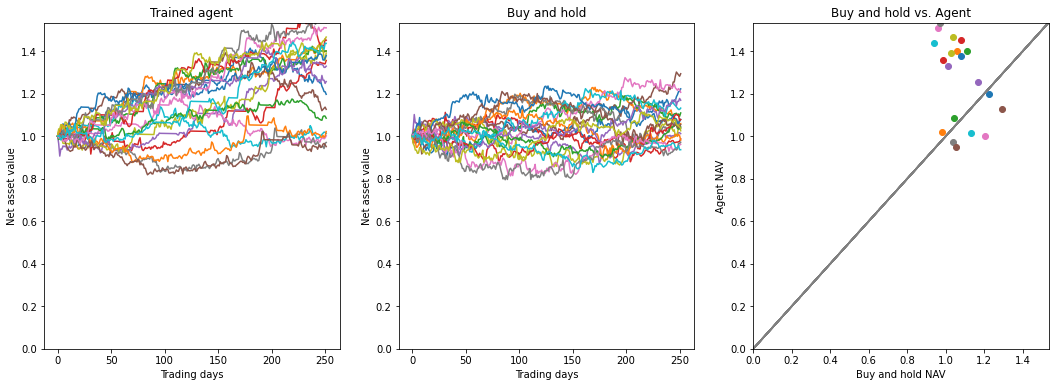
\includegraphics[width=0.78\textwidth]{z074_1.png}
  \caption{Toyota -- actions chosen by the trained agents over time.}
\end{figure}

\paragraph{Commentary on the result for Toyota.}
Given those numbers, it can be stated that the A2C algorithm applied to the Toyota share
would result in an overall better performance than the simple buy-and-hold strategy. In
78\% of the cases (on average) the trained agent would show a better performance. The
analysis of the performed actions shows different values for all trained agents. It can
therefore be assumed that the trained agent applied to this share could lead to
inconsistent behavior but could also lead to overall promising results.

\section{Technical Indicators}

\subsection{Relative Strength Index (RSI)}

The RSI indicator moves between zero and 100, plotting recent price gains versus recent
price losses. The RSI levels therefore help in estimating momentum and trend strength:
\begin{equation}
  RSI_t(n) = \frac{\sum_{k=0}^{n-1}(P_{t-i}-P_{t-i-1})\,\mathbb{1}\{P_{t-i}>P_{t-i-1}\}}{\lvert P_{t-1}-P_{t-i-1}\rvert}\times 100,
\end{equation}
where $RSI_t$ is the Relative Strength Index at time $t$, $P_t$ is the value of the index
at time $t$, and $n$ is the number of RSI periods. The RSI ranges from 0 to 100. A stock
is considered \emph{overbought} when its RSI is above 70, while it is regarded as
\emph{oversold} when the RSI is below 30.

\subsection{Moving Average Convergence Divergence (MACD)}

The MACD helps traders see the trend direction as well as the momentum of that trend. It
also provides a number of trade signals. When the MACD is above zero, the price is in an
upward phase; if the MACD is below zero, it has entered a bearish period. The indicator is
composed of two lines: the MACD line and a signal line, which moves slower. When the MACD
crosses below the signal line, it indicates that the price is falling; when the MACD line
crosses above the signal line, the price is rising. The MACD is constructed based on
moving averages: it is calculated by subtracting the longer exponential moving average
(EMA) from the shorter EMA. The EMA is defined as
\begin{equation}
  EMA_t = \frac{2}{n}\times(p_t - EMA_{t-1}) + EMA_{t-1},
\end{equation}
where $EMA_t$ is the exponential moving average at time $t$ and $n$ is the number of
periods for the EMA.

\subsection{On-Balance Volume (OBV)}

The on-balance volume indicator measures the positive and negative flow of volume over
time. It is calculated using the closing price and the trading volume of a stock.
Mathematically, the OBV of a stock at time $t$ is defined as
\begin{equation}
  OBV_t =
  \begin{cases}
    OBV_{t-1} + V_t, & C_t > C_{t-1},\\[2pt]
    OBV_{t-1} - V_t, & C_t < C_{t-1},
  \end{cases}
\end{equation}
where $C_t$ and $V_t$ are the closing price and the trading volume, respectively, at time
$t$. By definition, the OBV increases when prices rise and vice versa.

\subsection{Aroon Indicator}

The Aroon indicator measures whether the price is hitting new highs or lows over the
calculation period (typically 25). The formula for the Aroon oscillator is
\begin{align}
  Aroon\ Oscillator &= Aroon\ Up - Aroon\ Down,\\
  Aroon\ Up &= 100\times\frac{25 - \text{periods since 25-period high}}{25},\\
  Aroon\ Down &= 100\times\frac{25 - \text{periods since 25-period low}}{25}.
\end{align}
When the Aroon Up crosses above the Aroon Down, that is the first sign of a possible trend
change. If the Aroon Up hits 100 and stays relatively close to that level while the Aroon
Down stays near zero, that is positive confirmation of an uptrend.

\subsection{Stochastic Oscillator}

The stochastic oscillator measures the current price relative to the price range over a
number of periods. Plotted between zero and 100, the idea is that when the trend is up,
the price should be making new highs; in a downtrend, the price tends to make new lows.
The stochastic tracks whether this is happening:
\begin{align}
  CL_t &= P_t - \min(P_t, P_{t-1}, \dots, P_{t-s}),\\
  HL_t &= \max(P_t, P_{t-1}, \dots, P_{t-8}) - \min(P_t, P_{t-1}, \dots, P_{t-8}),\\
  RSV  &= \frac{CL_t}{HL_t}\times 100,\\
  K_t  &= \frac{2}{3}K_{t-1} + \frac{1}{3}RSV_t,\\
  D_t  &= \frac{2}{3}D_{t-1} + \frac{1}{3}K_t,
\end{align}
where $CL_t$ is measured as the lowest closing price in $N$ recent days subtracted from the
latest closing price; $HL_t$ refers to the difference between the highest and the lowest
closing price within $N$ days; $RSV_t$ is the $CL_t$ over the $HL_t$; the $K$ value is the
sum of $1/3$ of the $RSV$ value and $2/3$ of the $K$ value at lag one; and the $D$ value is
the sum of $1/3$ of the $K$ value and $2/3$ of the $D$ value at lag one. According to the
above equations, the $K$ and $D$ values range from 0 to 100. Overbought signals are emitted
as $K>80$ and $K>D$; oversold signals are emitted as $K<20$ and $K<D$.

\subsection{Comments}

\begin{figure}[H]
  \centering
  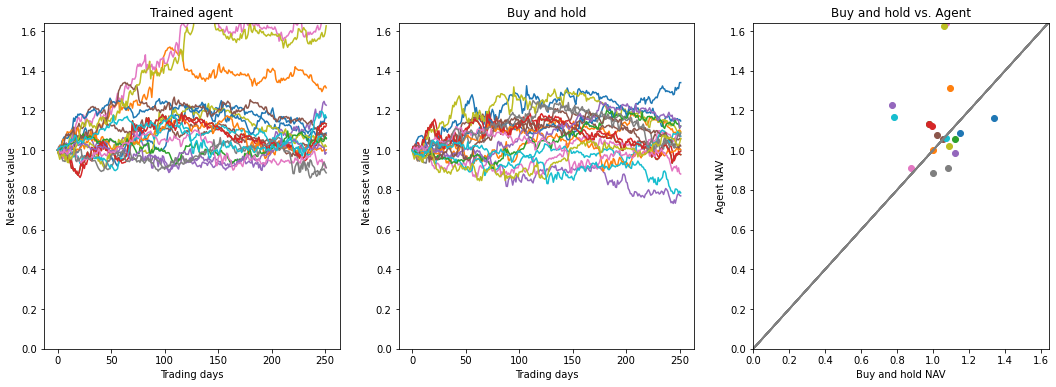
\includegraphics[width=0.78\textwidth]{z108_1.png}
  \caption{Selected technical indicators -- comparison of revenues, buy and hold vs.\ agent.}
\end{figure}

\begin{figure}[H]
  \centering
  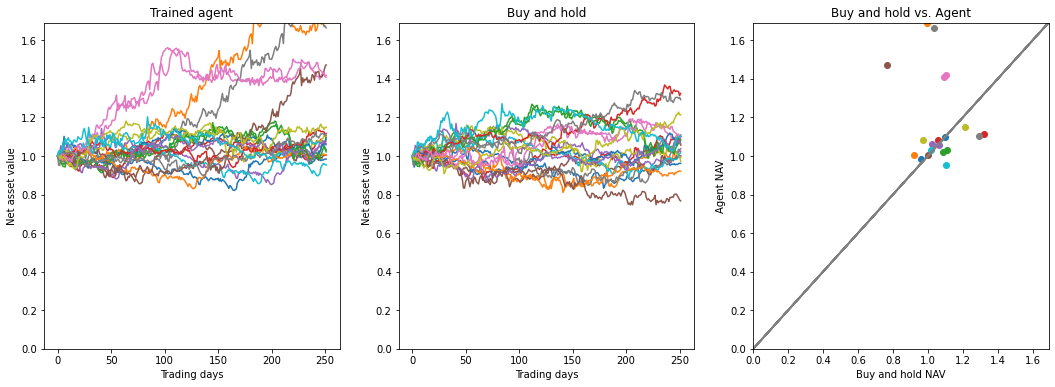
\includegraphics[width=0.78\textwidth]{z109_1.png}
  \caption{Selected technical indicators -- actions chosen by the trained agents over time.}
\end{figure}

Comparing the graphs on the ratio of revenues between buy and hold and the trained agent,
it is obvious that the revenues are similarly distributed, so there is no advantage for
one of the strategies. However, the actions chosen over time give an insight into the fact
that the trained agents suggest clearly different decisions. It can therefore be assumed
that the trained agent applied to this share could lead to inconsistent behavior.
Comparing those results with the agent trained with all indicators from above, it is well
evident that in both described categories no better result can be achieved by only using
the 5 indicators I selected.

\section{Correlated State Variables}

As an alternative to using all technical indicators, the 11 indicators that correlate most
with tomorrow's log-return of the closing price were selected as state variables. This
reduces the dimensionality of the state space while aiming to retain the most informative
features.

\begin{figure}[H]
  \centering
  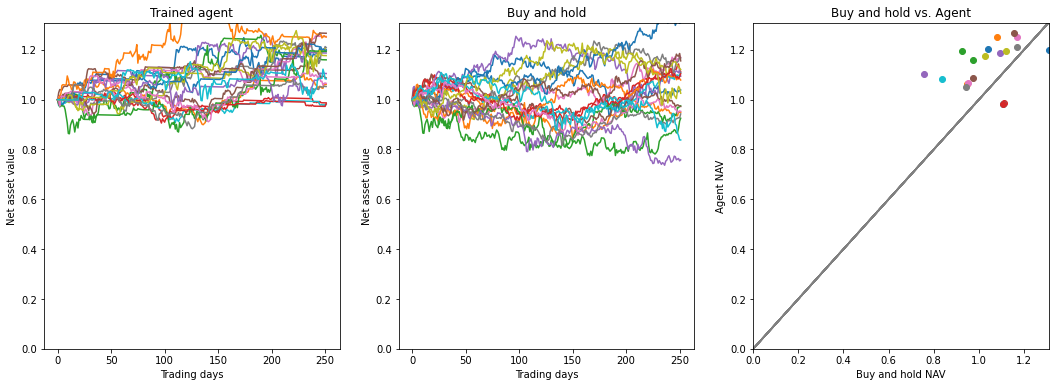
\includegraphics[width=0.78\textwidth]{z122_1.png}
  \caption{Correlated state variables -- cumulative return ratio: buy and hold vs.\ agent.}
\end{figure}

\begin{figure}[H]
  \centering
  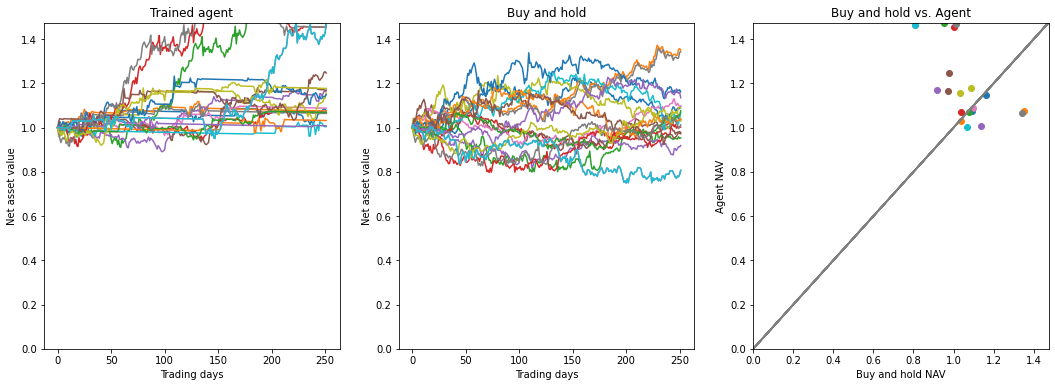
\includegraphics[width=0.78\textwidth]{z123_1.png}
  \caption{Correlated state variables -- actions chosen by the trained agents over time.}
\end{figure}

\paragraph{Comments.}
Comparing the graphs on the ratio of revenues between buy and hold and the trained agent,
it is obvious that the revenues are clearly better for the trained agent in comparison to
buy and hold. However, the actions chosen over time give an insight into the fact that the
trained agents suggest clearly different decisions. It can therefore be assumed that the
trained agent applied to this share could lead to inconsistent behavior. Comparing those
results with the agent trained with all indicators from above, it is evident that in the
case of positive revenues, the trained agent using the 11 indicators that correlate most
with tomorrow's log-return of the close price provides similar results as the one using
all indicators.

\section{Test Trained Agent on Different Time Periods}

The data is divided into train sets and test sets according to the trading time. After the
agents are trained over a specified timeframe, they are then evaluated on the test set
consisting of a different timeframe.

\begin{figure}[H]
  \centering
  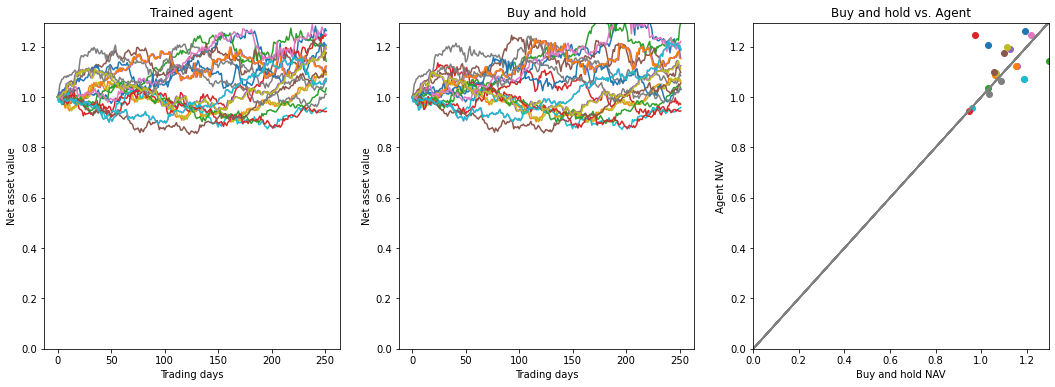
\includegraphics[width=0.78\textwidth]{z129_1.png}
  \caption{Train/test split -- cumulative return ratio (split 1).}
\end{figure}

\begin{figure}[H]
  \centering
  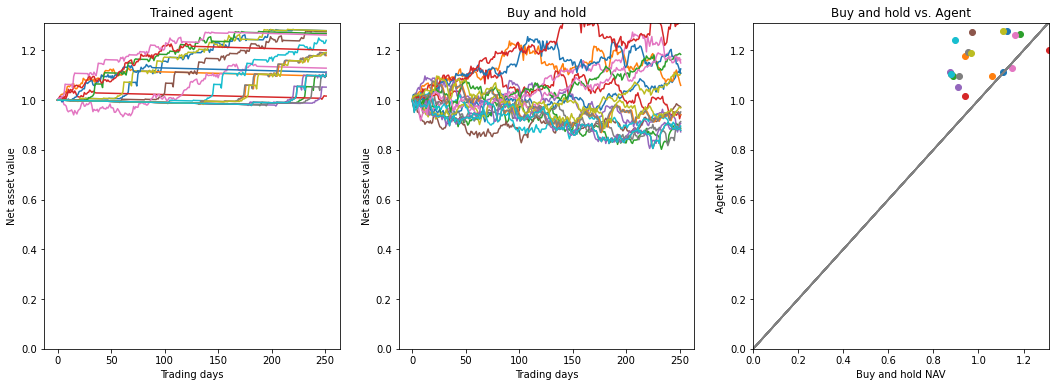
\includegraphics[width=0.78\textwidth]{z130_1.png}
  \caption{Train/test split -- cumulative return ratio (split 2).}
\end{figure}

\begin{figure}[H]
  \centering
  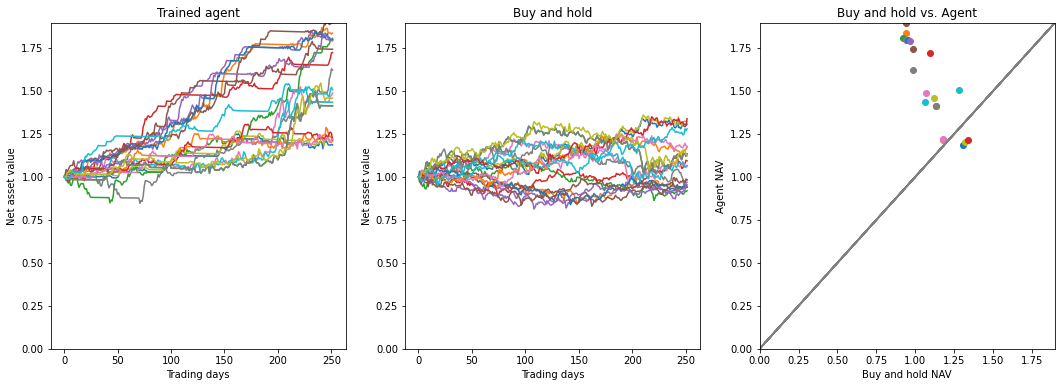
\includegraphics[width=0.78\textwidth]{z132_1.png}
  \caption{Train/test split -- cumulative return ratio (split 4).}
\end{figure}

\paragraph{Comments.}
Results show that even when the trained agent shows promising results in terms of profits,
if applied on the test set (except for one trained agent), positive rewards turn into
negative rewards. Even if they show consistent behavior, the outcome isn't.

As a central conclusion, two things can be stated:
\begin{itemize}
  \item If the agent is only trained over 4 years, no reliable predictions can be made
        about future behavior.
  \item The algorithm used here offers no possibility of predictability for future
        behavior in the field of stock trading and, on the contrary, performs worse than
        simple buy and hold.
\end{itemize}

\section{Overall Findings and Limitations}

The great advantage of RL is that an agent is able to learn and to perform actions in a
dynamically changing environment. It thus allows the best possible decisions to be made
during specific predefined points in time. The ability to train and improve the policy
independently through several iteration steps therefore allows an optimal applicability in
the field of algorithmic trading strategies. At the same time, the trading environment is
characterized by more or less external influences such as the size and thus the power of
larger investors, the influence of news and daily developments, decisions of individual
investors, etc. It can further be assumed that the generalizability of an RL model is
difficult to realize and it can therefore be a challenge to derive clear future behavioral
implications.

Applied to my example, I could show that, for example, the application of the A2C
algorithm to the Boeing stock over the last 10 years would lead to an average negative
reward compared to a simple buy-and-hold strategy over the same period. This could be
explained by the fact that especially drastic external influences have led the stock to
behave in an unusual way. Out of 5 trained agents, one in particular showed very poor
results of less than 1, which supports my thesis of the time dependency and volatility of
the model. Nevertheless, for the other two stocks of Airbus and Toyota over a time period
of 10 years, the algorithm showed significantly better results in some cases, but without
outputting consistent behavior once the agent is trained several times. It is further
interesting to note that results in terms of positive rewards do not deviate much when all
technical indicators are used on the one hand and only the 11 indicators that correlate
most with tomorrow's log-return of the close price on the other.

By training the agent on the Toyota stock and then testing the model over a different time
period, I was able to show that the algorithm used on this stock is unlikely to generate
promising results in the future.

\section{Summary on One Selected Paper}

\subsection{Deep Robust Reinforcement Learning for Practical Algorithmic Trading}
\textit{Yang Li, Wanshan Zheng and Zibin Zheng (2019)}

In their 2019 paper, Yang Li, Wanshan Zheng and Zibin Zheng present a further development
of previously used RL algorithms such as A3C and DQN for application in stock trading, a
so-called \emph{deep robust reinforcement learning} framework. To cope with the problem of
uncontrollable external influences, called \emph{noise} in their study, the following steps
have to be performed first:
\begin{itemize}
  \item Sampling random lengths of time units.
  \item To limit the influence of news, which is usually highest at opening time, the time
        points between 9:30 am to 11:30 am and 13:00 pm to 15:00 pm are omitted.
  \item Removal of the low volatility from the calculation in order to mitigate the effect
        caused by individual investors (as opposed to institutional investors).
\end{itemize}

In addition, to further reduce noise, the method of so-called SDAEs is utilized. The result
of the last hidden layer is then fed into a LSTM layer in order allowing the agent to
resolve the partial observability and discover latent patterns. For the model 5 stocks were
chosen (3 NASDAQ, 1 S\&P 500 stock index mini future, 1 HS300 stock index future). The
results applied on their test set show that both algorithms output significantly better
results in terms of annualized returns than both the original A3C and DQN algorithms as well
as simple buy and hold. Furthermore, their study shows that the SDAEs-LSTM A3C algorithm
performs significantly better than the SDAEs-LSTM DQN algorithm across all stocks.

\noindent\textit{Y. Li, W. Zheng and Z. Zheng, ``Deep Robust Reinforcement Learning for
Practical Algorithmic Trading,'' in IEEE Access, vol.~7, pp.~108014--108022, 2019,
doi: 10.1109/ACCESS.2019.2932789.}

\subsection{Related Work: Three Answers to the Generalization Problem}
\label{sec:related-work}

The three papers read for this report attack the same difficulty -- the gap between
in-sample fit and out-of-sample performance -- from three different sides, and all three
support the central observation of the 2026 update.

\paragraph{Representation.} Li, Zheng and Zheng (2019) change the input side of the agent:
stacked denoising autoencoders (SDAEs) clean the noisy market data and an LSTM layer
resolves the partial observability of the market state. On ten years of minute data their
extended DQN and A3C variants beat the plain algorithms and buy-and-hold in annualized
return. Their evaluation, however, still rests on a single 90/10 train--test split, so the
reported edge is an in-sample statement in the sense of our own comparison.

\paragraph{Environment.} Kuo et al.\ (2021) change the training environment instead of the
network. A LOB-GAN learns the ordering behaviour of the limit order book; its generator,
combined with a matching engine, forms an interactive ``Virtual Market'' in which the
portfolio agent is trained. Training in this simulated market improves out-of-sample
portfolio performance by about four percent over other generalization strategies. This is
the mirror image of our own result: a static environment built from historical prices is
itself part of the generalization problem.

\paragraph{Policy.} Niu, Li and Li (2022) keep the environment and diversify the policy set.
MetaTrader first imitates several expert strategies (momentum, mean reversion, hindsight) to
obtain a set of diverse base policies, and then trains a DQN meta-policy that recognises the
current market regime and switches to the most suitable base policy. On DJIA, HSI and CSI100
it reports clearly better risk-adjusted returns than DeepTrader and the classical
strategies.

Our own re-run (Chapter~\ref{sec:update-a2c} and the 20-seed extension in the accompanying
update report) sits between these three positions: the representation is unchanged (no
SDAE), the environment is still built from historical prices, and the policy set is a single
A2C agent. What was made robust instead is the evaluation itself -- every configuration was
repeated with twenty seeds. The outcome is sober and matches the papers' implicit lesson:
in-sample the agent wins clearly on all three stocks, but out-of-sample only Boeing keeps a
significant edge over buy-and-hold, Airbus ends exactly on buy-and-hold and Toyota turns
significantly worse. The in-sample margin does not predict the out-of-sample result. Read
against the three papers, this suggests that robustness has to be built into the
representation, the environment or the policy ensemble; a single-agent, single-environment
setup like ours should not be expected to generalise on its own.

\noindent\textit{C.-H. Kuo, C.-T. Chen, S.-J. Lin and S.-H. Huang, ``Improving Generalization
in Reinforcement Learning-Based Trading by Using a Generative Adversarial Market Model,'' in
IEEE Access, vol.~9, 2021, doi: 10.1109/ACCESS.2021.3068269.}

\noindent\textit{H. Niu, S. Li and J. Li, ``MetaTrader: A Reinforcement Learning Approach
Integrating Diverse Policies for Portfolio Optimization,'' in Proc.\ 31st ACM Int.\ Conf.\ on
Information and Knowledge Management (CIKM '22), Atlanta, GA, USA, 2022,
arXiv:2210.07771.}

\section{2026 Update: Fundamentals and a Re-run of the A2C Part}

This chapter extends the original project with data up to 6 October 2026. It has two parts:
an update of the fundamental figures (Section~\ref{sec:update-fundamentals}) and an
independent re-run of the reinforcement-learning part on the new data window
(Section~\ref{sec:update-a2c}). The re-run had to be carried out in a different software
environment than the original notebook; every deviation is documented in
Section~\ref{sec:update-deviations} and should be read before comparing any number.

\subsection{Updated Fundamental Figures}
\label{sec:update-fundamentals}

Methodology as in Chapter~1: P/E and P/S are trailing values, and the log-return is the sum
of the daily log-returns of the adjusted close over twelve months.

\begin{table}[H]
  \centering
  \caption{Fundamental figures: original notebook (2022) versus 6 October 2026.}
  \label{tab:update-fundamentals}
  \begin{tabular}{lrrr}
    \toprule
    Figure & Boeing (BA) & Airbus (AIR.PA) & Toyota (TM)\\
    \midrule
    P/E 2022        & n/a (KeyError) & 19.887 & 10.375\\
    P/E 2026        & 70.79          & 25.04  & 7.91\\
    P/S 2022        & 1.502          & 1.458  & 0.0063\\
    P/S 2026        & 1.60           & 1.93   & 0.68\\
    Log-return 2022 & $-0.3025$      & $-0.1451$ & $-0.1486$\\
    Log-return 2026 & $-0.1558$      & $-0.0945$ & $-0.0743$\\
    \bottomrule
  \end{tabular}
\end{table}

\paragraph{P/E ratio.} The statement from Section~1.2 is confirmed and partly sharpened.
Airbus remains above the guideline value of 15 (19.9 $\rightarrow$ 25.0), Toyota clearly
below it (10.4 $\rightarrow$ 7.9). Boeing delivers a value for the first time: \textbf{70.79},
which is an extremely high valuation multiple -- a statement about valuation, not about the
share price.

\paragraph{P/S ratio.} The update uncovered a data error in the original notebook. The value
of $0.0063$ reported for Toyota (interpreted there as ``close to zero'', i.e.\ very cheap) was
a \texttt{yfinance} outlier. The actual value is \textbf{0.68}: Toyota is still the cheapest of
the three, but the original statement ``close to zero'' is wrong. Boeing stands at 1.60 and
Airbus at 1.93.

\paragraph{Log-returns.} The core statement holds: all three shares are negative over the last
twelve months as well (BA $-15.6\,\%$, AIR $-9.5\,\%$, TM $-7.4\,\%$), so buy-and-hold would
have lost money again. Over the longer horizon since the original data ended (August 2022),
however, all three are clearly positive (BA $+20.5\,\%$, TM $+39.5\,\%$, AIR $+50$ to
$+65\,\%$ over five years). The loss picture was therefore \emph{window-specific}.

\begin{figure}[H]
  \centering
  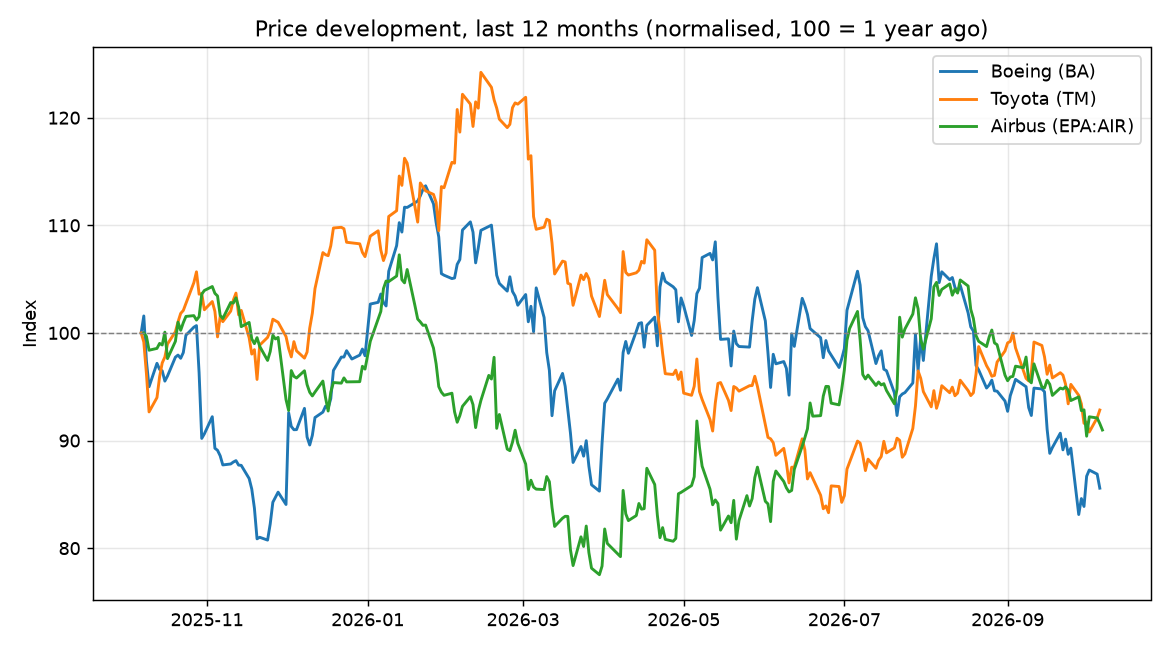
\includegraphics[width=0.80\textwidth]{update_2026_1y.png}
  \caption{Price development of the three shares over the last twelve months
  (normalised, 100 = one year ago).}
\end{figure}

\subsection{Re-run of the A2C Part on New Data}
\label{sec:update-a2c}

The protocol of the original notebook is reproduced: five agents with
\texttt{A2C("MlpPolicy")}, 75{,}000 timesteps each, evaluated with
\texttt{ai\_trade\_performance(num\_plays=20)}. The test environment re-uses the feature list
and the scaler of the training environment. Agent and buy-and-hold are evaluated on the same
twenty episode seeds, so the comparison is fair.

\begin{table}[H]
  \centering
  \caption{2026 re-run on Boeing: final NAV per episode (start $=1.0$), mean over
  twenty episodes per agent.}
  \label{tab:update-a2c}
  \begin{tabular}{crrr|rrr}
    \toprule
    \# & Seed & Train agent & Train B\&H & Test agent & Test B\&H & Test agent better\\
    \midrule
    1 & 100 & 1.6705 & 0.9647 & \textbf{0.5616} & 0.9475 & 0\,\%\\
    2 & 101 & 2.4073 & 0.9671 & 1.2403 & 0.9408 & 100\,\%\\
    3 & 102 & 4.0534 & 0.9956 & 0.9828 & 0.9412 & 75\,\%\\
    4 & 103 & 7.0580 & 0.9711 & 1.0106 & 0.9493 & 70\,\%\\
    5 & 104 & 5.1547 & 0.9727 & 1.1326 & 0.9485 & 80\,\%\\
    \midrule
    $\varnothing$ & & 4.0688 & 0.9742 & 0.9856 & 0.9455 & 65\,\%\\
    \bottomrule
  \end{tabular}
\end{table}

Training window 6 October 2021 to 31 May 2024 (in-sample), test window 1 June 2024 to
6 October 2026 (out-of-sample).

\paragraph{In-sample results are not evidence of skill.} On the training window the agents
reach an average NAV of 4.07 against 0.97 for buy-and-hold, and they beat the benchmark in
every episode. This is not a result -- the agents were trained on exactly this window, so the
figure only shows that they memorised it.

\paragraph{Out-of-sample the picture is sober.} On the test window the average NAV is 0.9856
against 0.9455 for buy-and-hold, with the agent ahead in \textbf{65\,\%} of the episodes --
but with a very wide spread: agent 1 loses heavily (0.56), agent 2 wins clearly (1.24), and
two of five agents lose against buy-and-hold in at least a quarter of the episodes. The
advantage lies within seed variance and is \textbf{not significant}.

\paragraph{Buy-and-hold is below 1.0 in both windows}, i.e.\ Boeing lost value over both
periods. The question here is therefore ``lose less'', not ``win''. Overall the re-run
\textbf{supports} the conclusion of the original notebook: A2C does not deliver a reliable
outperformance.

\begin{figure}[H]
  \centering
  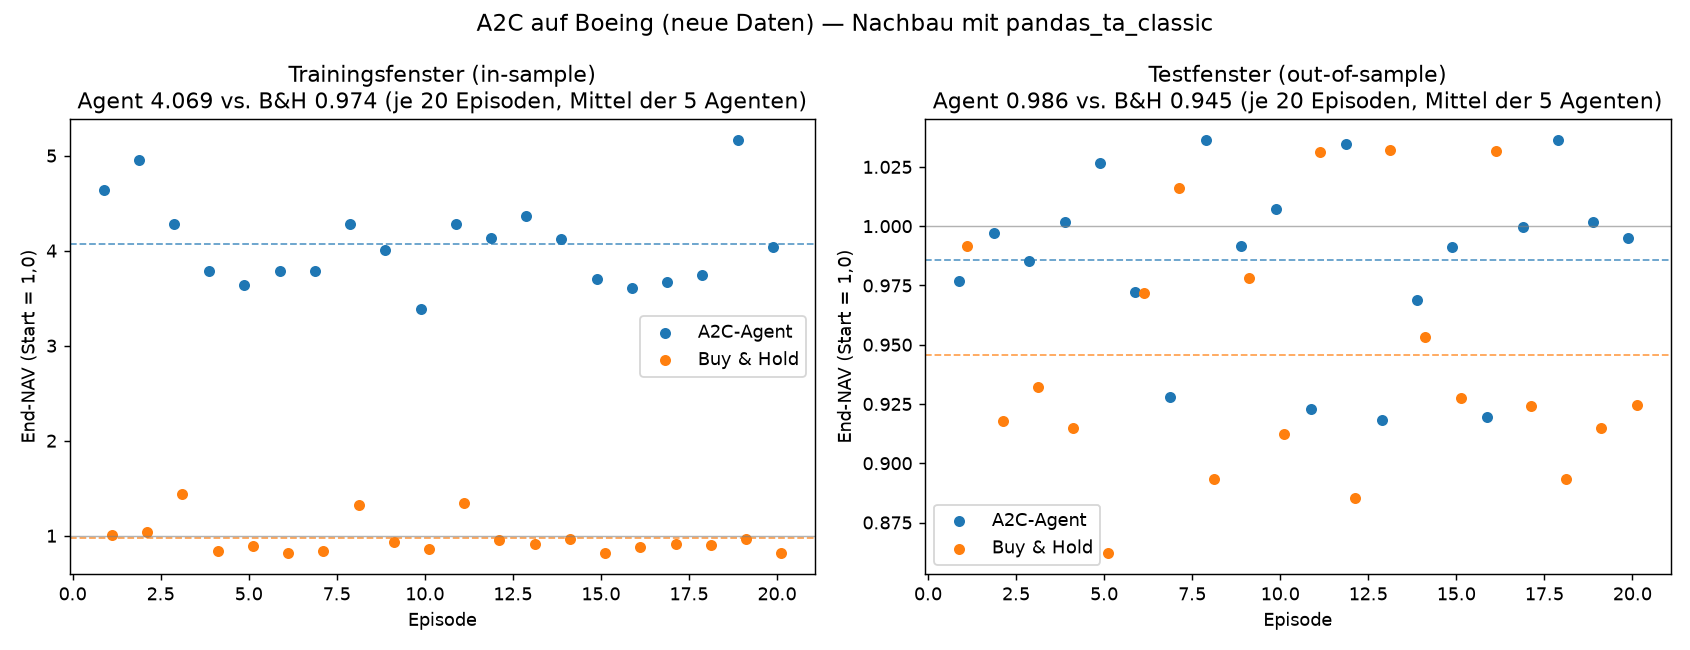
\includegraphics[width=0.95\textwidth]{update_2026_a2c.png}
  \caption{Final NAV per episode (mean of the five agents), left: training window
  (in-sample), right: test window (out-of-sample).}
\end{figure}

\begin{table}[H]
  \centering
  \caption{Action distribution of the agents (one episode each).}
  \label{tab:update-actions}
  \begin{tabular}{crrr|rrr}
    \toprule
    \# & Train short & Train cash & Train long & Test short & Test cash & Test long\\
    \midrule
    1 & 268 & 18  & 348 & 239 & 17  & 299\\
    2 & 295 & 39  & 300 & 304 & 24  & 227\\
    3 & 297 & 24  & 313 & 279 & 29  & 247\\
    4 & 246 & 212 & 176 & 260 & 201 & 94\\
    5 & 296 & 15  & 323 & 309 & 12  & 234\\
    \bottomrule
  \end{tabular}
\end{table}

All agents trade predominantly long; only agent~4 holds a large cash position. Short
positions are almost always held, but rarely with a large weight.

\subsection{Deviations from the Original Notebook}
\label{sec:update-deviations}

The re-run did not execute in the original conda environment (Python 3.8.8,
stable-baselines3 1.6.0, gym 0.21, torch 1.12.1) but in a Linux container with a current
stack. All substitutions are deliberate and documented.

\begin{table}[H]
  \centering
  \caption{Substitutions in the 2026 re-run.}
  \label{tab:update-deviations}
  \begin{tabular}{lll}
    \toprule
    Aspect & Original notebook & 2026 re-run\\
    \midrule
    Price data       & \texttt{yfinance} (live)   & local CSV\\
    Technical indicators & \texttt{pandas\_ta} 0.3.14b0 & \texttt{pandas\_ta\_classic}\\
    Indicator count  & 204                        & 348\\
    Observation size & 205                        & \textbf{334}\\
    Parallelisation  & multiprocessing pool       & serial\\
    RL stack         & SB3 1.6.0 + gym 0.21       & SB3 2.9 + gymnasium 1.4\\
    \bottomrule
  \end{tabular}
\end{table}

\textbf{The most important limitation is the observation size of 334 instead of 205.} The
agent sees more input features than in the original, so part of any performance difference
may stem from that and not from the data update. In addition, \texttt{yfinance} is blocked
from this host (HTTP~429 on every endpoint), which is why the price series is read from a
local file, and the helper package \texttt{aif\_course} is no longer
available (the upstream repository returns HTTP~404). The environment had to be
reconstructed locally; the exact substitutions are documented in the accompanying code.

\subsection{Conclusion of the Update}

The fundamental figures confirm the original assessment of Airbus (expensive) and Toyota
(cheap), correct the erroneous Toyota P/S value, and add a very high P/E for Boeing. The
loss picture of the log-returns is confirmed for the last twelve months, but turns out to be
window-specific over a longer horizon. The A2C re-run on new data reproduces the original
conclusion: on average the agent is slightly ahead of buy-and-hold out-of-sample, but the
spread across seeds is so large that no reliable outperformance can be claimed.

\section{A3C: A Second Algorithm, a Decomposition and a Generative Market Model}
\label{sec:update-a3c}

\paragraph{Where the question comes from.} The original notebook and the re-run
(Section~\ref{sec:update-a2c}) use \emph{A2C}, i.e.\ synchronous learning. The obvious
cross-check is \emph{A3C}: several workers collect rollouts in parallel and push their
gradients into a shared network (Hogwild style, only the optimiser step is locked).
Environment, windows, episode seeds and evaluation functions are left unchanged, so the
comparison measures the learning algorithm and not the surrounding machinery. The final
evaluation again runs over \textbf{20 seeds (100--119)}. One peculiarity up front: A3C was
built only \emph{after} the A2C part was finished, so there is no notebook template against
which the numbers could be mirrored.

\subsection{The Baseline Has No Edge}

\begin{table}[H]
  \centering
  \caption{A3C on Boeing, 20 seeds. Margin $=$ agent $-$ buy-and-hold in NAV points
           (start $=1.0$); $p$ one-sided from the $t$-test ``margin $>0$''.
           ``R/R'' is the return/risk ratio in the test window.}
  \label{tab:update-a3c-arms}
  \small
  \begin{tabular}{lrrrrrr}
    \toprule
    Arm & Training & Test & 95\,\% CI test & Hit rate test & $p$ & R/R test\\
    \midrule
    Baseline                 & $+8.43$ & $+0.019$ & $[-0.06;+0.10]$ & 51.0\,\% & $0.32$  & $-0.24$\\
    \texttt{ent\_coef} 0.02  & $+8.37$ & $+0.047$ & $[-0.03;+0.12]$ & 64.0\,\% & $0.10$  & $-0.37$\\
    \texttt{obs\_noise} 0.01 & $+8.79$ & $+0.038$ & $[-0.03;+0.11]$ & 57.2\,\% & $0.14$  & $-0.45$\\
    \texttt{nstep} 10        & $+6.71$ & $+0.125$ & $[+0.01;+0.24]$ & 67.8\,\% & $0.019$ & $-0.05$\\
    Bundle (all three)       & $+7.69$ & $+0.145$ & $[+0.03;+0.26]$ & 70.2\,\% & $0.007$ & $-0.03$\\
    Bundle $+$ bootstrap     & $+0.02$ & $+0.218$ & $[+0.09;+0.35]$ & 77.8\,\% & $0.0012$& $+0.50$\\
    \texttt{nstep} 10 $+$ bootstrap & $+0.02$ & $+0.218$ & $[+0.09;+0.35]$ & 72.5\,\% & $0.0010$& $+0.38$\\
    \bottomrule
  \end{tabular}
\end{table}

The baseline repeats the A2C result: in the test window the margin is $+0.019$ NAV points,
the agent wins in \textbf{51.0\,\%} of the episodes --- a coin flip --- and the one-sided
$p$-value is $0.32$. \textbf{An unmodified A3C agent has no demonstrable edge over
buy-and-hold.} In the training window, at the same time, the margin is $+8.43$: the agent
has memorised the one historical path.

\subsection{Decomposition: Which Factor Carries the Effect?}

The obvious move is a bundle of three changes: \texttt{nstep} $5\to10$ (n-step returns),
\texttt{ent\_coef} $0.01\to0.02$ (entropy bonus) and \texttt{obs\_noise} $0\to0.01$
(Gaussian noise on the observation during training). The bundle lifts the test margin to
$+0.145$ ($p=0.007$). The only question is: \emph{which} of the three factors does that?

Each factor was therefore run on its own, again with 20 seeds (rows 2--4 of
Table~\ref{tab:update-a3c-arms}). The result is unambiguous and was surprising to me:

\paragraph{\texttt{nstep} is the active ingredient.} On its own, \texttt{nstep} $10$
already reaches $+0.125$ ($p=0.019$, hit rate 67.8\,\%) --- that is \textbf{85\,\%} of the
bundle's effect. The paired test bundle against \texttt{nstep} alone gives $+0.020$ at
$p=0.81$: statistically \textbf{indistinguishable}. The bundle is therefore not a sum of
levers but essentially \texttt{nstep} plus noise.

\paragraph{\texttt{ent\_coef} and \texttt{obs\_noise} are inert.} On their own they yield
$+0.047$ ($p=0.64$) and $+0.038$ ($p=0.72$) against the baseline, with 10 and 9 of 20
positive seed differences respectively --- a coin flip. They do not act on the overfitting
either: the in-sample margin stays at $+8.37$ and $+8.79$ against $+8.43$ for the baseline
($p=0.90$ and $0.53$). Only \texttt{nstep} $10$ lowers it significantly to $+6.71$
($p=0.0015$) --- and at the same time raises the test value.

\paragraph{Additivity.} The sum of the three single deltas is $+0.155$, the bundle sits at
$+0.126$; the residual is $-0.029$ against a spread of $0.61$ ($p=0.84$). The point
estimate is thus slightly sub-additive ($0.82\times$), but statistically indistinguishable
from pure additivity --- the noise dominates. There is no synergy in any case.

\subsection{A Generative Market Model Instead of Rolling Windows}

The second idea comes from the paper selection (Kuo et al., LOB-GAN, see
Chapter~\ref{sec:related-work}): does the agent generalise better if it sees \emph{several
plausible market paths} instead of a single historical one? The obvious route would be
rolling training windows --- and that is \textbf{not buildable} in this protocol. The
environment forces more than $2 \cdot 252 = 504$ observations per environment
(\texttt{assert len(df) > 2*trading\_days}), and \texttt{trading\_days} simultaneously sets
the episode length of 252 steps; the minimum therefore cannot be lowered without breaking
the protocol. The training window, however, has only \textbf{634} usable rows, and the price
series starts exactly at the window's beginning. Two genuine sub-windows would each need
around 550 rows --- impossible. The code now checks this itself and aborts with a clear
message.

Instead, a \textbf{block bootstrap} generates synthetic price series. What matters is
\emph{what} is resampled: price levels would be wrong, because every block seam would create
an artificial jump (a block ends at 100, the next starts at 80 --- minus 20\,\% overnight).
The \emph{daily shape} is therefore bootstrapped:
$\log(\text{Close}_t/\text{Close}_{t-1})$, $\log(\text{Open}_t/\text{Close}_{t-1})$,
$\log(\text{High}_t/\text{Close}_t)$, $\log(\text{Low}_t/\text{Close}_t)$ and
$\log(\text{Volume}_t)$. Blocks of 20 consecutive days are drawn with replacement and the
path is rebuilt from the first real close. Within the blocks the autocorrelation is
preserved, the curve is continuous by construction, and the agent never sees the \emph{real}
training path. Cross-check: the spread of the daily returns is $0.0229$ and $0.0247$ in the
synthetic series against $0.0239$ in the real series.

\subsection{Isolation: the Bootstrap Carries, the Two Passengers Do Not}

In the ``bundle $+$ bootstrap'' row the bootstrap still sits together with the two inert
factors. The isolating run \texttt{nstep} $10$ $+$ bootstrap without \texttt{ent\_coef} and
\texttt{obs\_noise} closes that gap (last row):

\begin{table}[H]
  \centering
  \caption{Paired tests over the 20 seed differences (df$=19$), test margin.}
  \label{tab:update-a3c-paired}
  \small
  \begin{tabular}{lrrr}
    \toprule
    Comparison & $\Delta$ test margin & $t$ & $p$\\
    \midrule
    \texttt{nstep} 10 $-$ baseline            & $+0.107$ & $1.69$ & $0.107$\\
    \texttt{ent\_coef} 0.02 $-$ baseline      & $+0.028$ & $0.47$ & $0.643$\\
    \texttt{obs\_noise} 0.01 $-$ baseline     & $+0.020$ & $0.36$ & $0.720$\\
    bundle $-$ baseline                       & $+0.126$ & $1.98$ & $0.062$\\
    bundle $-$ \texttt{nstep} 10              & $+0.020$ & $0.24$ & $0.810$\\
    \texttt{nstep} 10 $+$ bootstrap $-$ baseline & $+0.200$ & $2.35$ & $\mathbf{0.030}$\\
    \texttt{nstep} 10 $+$ bootstrap $-$ \texttt{nstep} 10 & $+0.093$ & $1.16$ & $0.260$\\
    \texttt{nstep} 10 $+$ bootstrap $-$ bundle $+$ bootstrap & $+0.0002$ & $0.003$ & $0.998$\\
    \bottomrule
  \end{tabular}
\end{table}

\paragraph{The bootstrap effect survives in isolation --- and was never carried by the
passengers.} The isolated increment is $+0.093$ and thus \emph{exactly} the same value as
the contaminated estimate ($+0.093$); the ratio is $1.00$. The effect has therefore neither
shrunk nor disappeared. One caveat: on its own it is \textbf{not significant} ($p=0.26$,
12 of 20 seeds positive, median $+0.138$, trimmed mean $+0.112$) --- the point estimate is
stable, the sample is too small.

\paragraph{\texttt{nstep} 10 $+$ bootstrap is indistinguishable from ``bundle $+$
bootstrap''} ($+0.0002$, $p=0.998$). \texttt{ent\_coef} and \texttt{obs\_noise} are thus
\textbf{finally proven to be passengers}: the two runs differ only in those two parameters
and produce practically the same distribution. (Incidentally a consistency check that the
bootstrap replicates are deterministic.)

\paragraph{A significant edge for the first time.} \texttt{nstep} $10$ $+$ bootstrap is
significantly better than the baseline ($+0.200$, $p=0.030$) and its own test margin is
clearly different from zero ($p=0.0010$, two-sided $0.0019$). This is the \emph{first} arm
in this project to break the 5\,\% threshold in the paired test against the baseline ---
neither \texttt{nstep} alone ($p=0.107$) nor the bundle ($p=0.062$) manages that.

\begin{figure}[H]
  \centering
  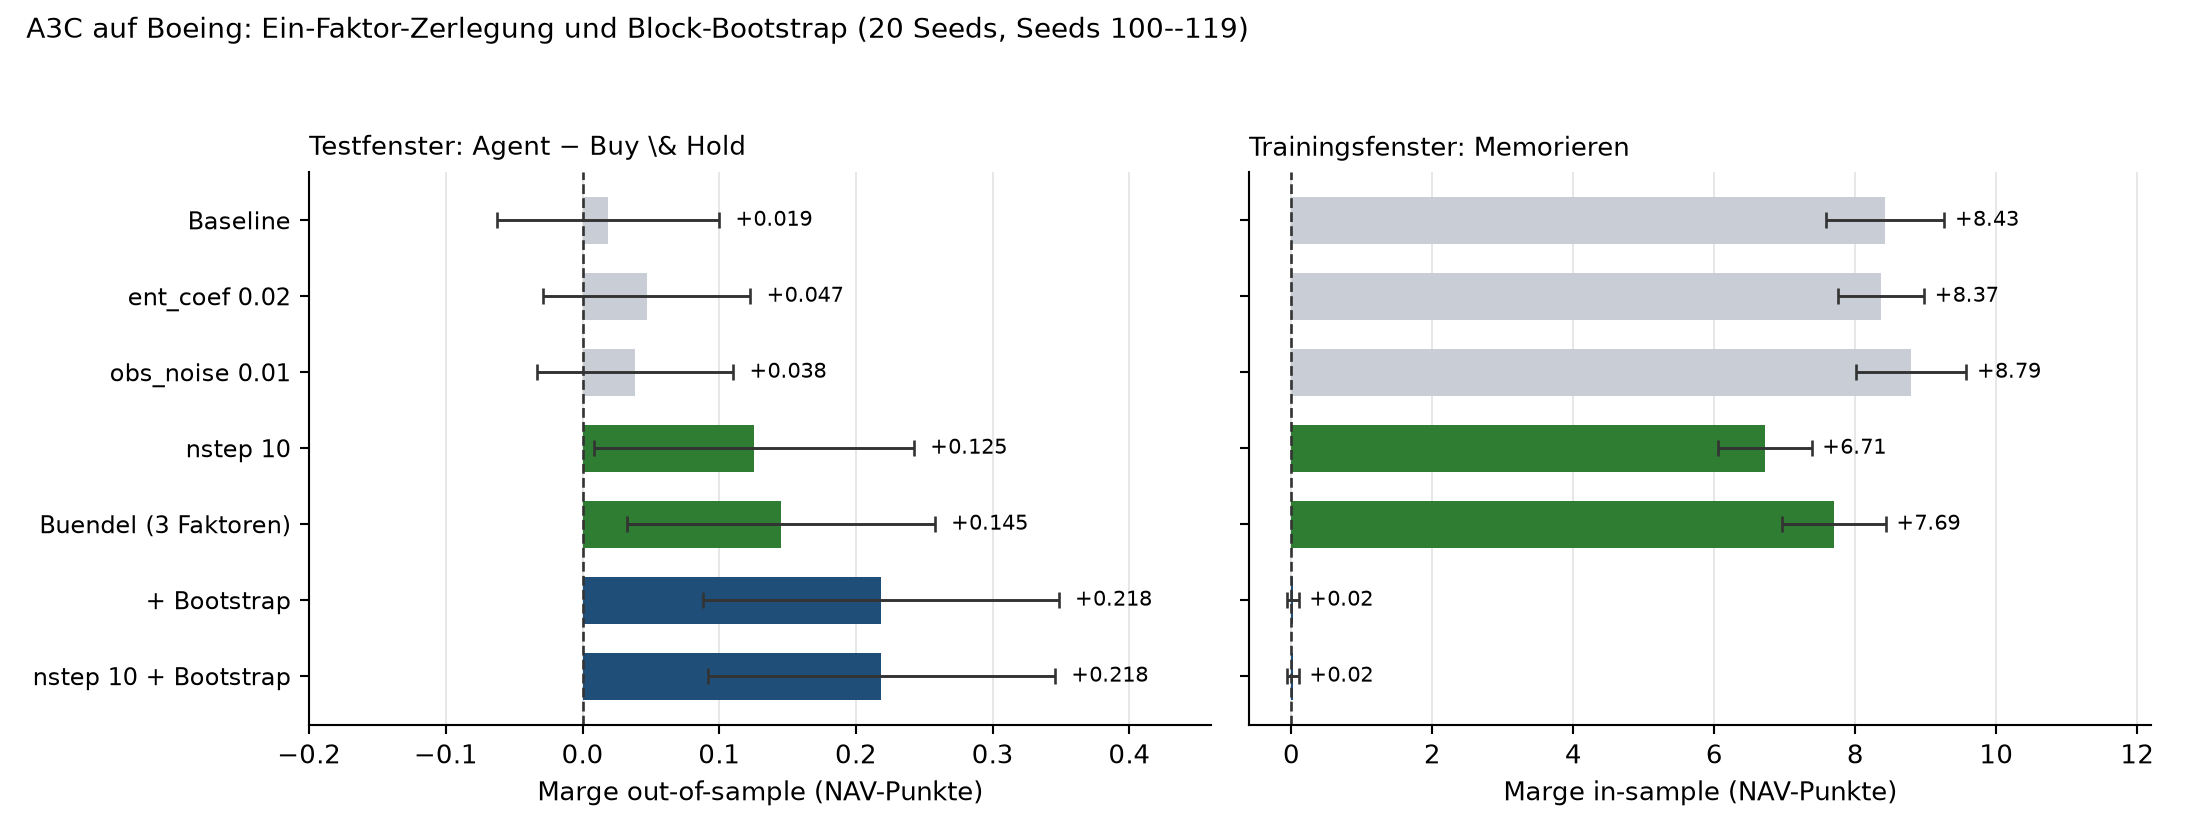
\includegraphics[width=\textwidth]{update_2026_a3c.png}
  \caption{One-factor decomposition and block bootstrap, 20 seeds. Left the test margin
  (error bars: 95\,\% CI), right the margin in the training window. The two bootstrap arms
  (dark) have practically zero in-sample edge and the largest out-of-sample one.}
  \label{fig:update-a3c}
\end{figure}

\subsection{What the Overfitting Picture Shows}

Figure~\ref{fig:update-a3c} makes the core visible. The four arms that train on the real
window carry an in-sample margin of between $+6.7$ and $+8.8$ NAV points --- and almost
none of it survives out-of-sample. The two bootstrap arms have an in-sample margin of
$+0.02$, i.e.\ \emph{zero} edge, and at the same time deliver the best test values. They
never saw the historical path; that they do not win in the training window is therefore not
a weakness but the mechanism. An in-sample edge of $+8$ is thus exposed as what it is:
memorisation.

\subsection{Limitations}

\paragraph{20 seeds are a small sample.} The confidence intervals in
Table~\ref{tab:update-a3c-arms} are wide, and the central bootstrap increment is
underpowered at $p=0.26$. What is robust: that the baseline has no edge, that
\texttt{nstep} $10$ explains the bundle, that the two remaining factors do nothing, and
that \texttt{nstep} $10$ $+$ bootstrap beats the baseline significantly. What is not robust
is the claim that the bootstrap addition is significant \emph{by itself}.

\paragraph{Only five different synthetic paths.} With 20 agents and five bootstrap
replicates, groups of four seeds share the same synthetic series. The seeds then vary only
the exploration, not the environment. A run with one path per agent would be the next clean
step.

\paragraph{The in-sample margin of the bootstrap arms is not comparable.} It is measured on
the real window, on which these agents never trained; the row is therefore readable only as
an overfitting indicator, not as a performance measure.

\paragraph{Data and environment.} The limitations from Section~\ref{sec:update-deviations}
apply: observation vector 334 instead of 205, local CSVs instead of \texttt{yfinance}. A3C
uses the same environment as A2C, so the deviations affect both arms equally.

\subsection{Conclusion of the A3C Part}

The baseline confirms the A2C finding on a second algorithm: no demonstrable edge over
buy-and-hold. The decomposition shows that the effect of the obvious ``regularisation''
actually comes from the \textbf{credit assignment} (\texttt{nstep} $5\to10$); entropy bonus
and observation noise are ineffective at this magnitude. The \textbf{block bootstrap}
delivers, as a second lever, the best test value and the first significant edge over the
baseline --- but only in combination. Conceptually this is the more interesting finding: the
agent does not need the real historical path to be level with or better than buy-and-hold on
the test window; many plausible paths are enough.


\appendix
\section{Notebook Code}

The complete Python code of the project notebook is listed below. It contains all data
acquisition, feature engineering, environment setup, training and evaluation steps in the
order in which they were executed in the Jupyter notebook.

\lstinputlisting[language=Python,caption={Complete code of the project notebook.}]{code/notebook_code.py}


\end{document}
